\section{\us}
\label{sec:simEngine}
%Our fundamental question in this work is 
To determine how similar proxy and parent applications behave in terms of resource utilization such as computation and memory, we explore the use of several ML similarity techniques. Those techniques work differently, making it hard to determine which one reveals the real relationship, so we create \us to intercept the level of agreement between those techniques that could reflect the accurate answer. 
%\todo{why we need to use several similarity techniques?}
%A fundamental question we pose is: ``how similar are applications to each other in the way they utilize system resources, particularly computation and memory?''
%, with a focus in this work on node computation and memory resources. 
%We introduce a framework \us to determine this similarity between proxy and parent applications.
%Figure~\ref{figs:us} shows the workflow of \us.

We collect hardware performance counters from several proxy, parent applications, and benchmarks to provide a comprehensive collection of informational measurements that reveals the application execution resources fingerprints.  
Figure~\ref{figs:us} shows the workflow of \us, where we use Lightweight Distributed Metric Service (LDMS)~\cite{ldms_sandia} as the data collection to collect HW performance counters from HPC applications. Then, LDMS send the data to the feature selection layer as a data matrix $X$ that has $n$ rows of application vectors $x_{1},\ldots,x_{n}$ and features $f_{1},\ldots,f_{d}$ as the columns.

%a vector $x_{i}$ with the length of $d$ dimensions ($d$ being the number of hardware events), and build a data matrix $X$ that has $n$ rows of application vectors $x_{1},\ldots,x_{n}$. The columns of $X$ are the features $f_{1},\ldots,f_{d}$.

During feature selection, we rank the features by calculating importance scores and select the important $k$ features by a correlation filter.
In this way, we find the subset of $k$ important features which preserve the similarity structure of the matrix $X'$. 
Finally, using the selected important features, we produce similarity matrices to compare the similarity between applications and quantify the fidelity of proxy and parent applications. The final result will be a similarity matrix. \todo{explain  matrix content}
%Our analysis tools that compute feature ranking, correlation filter, and similarity measurement are written in python and use several of the standard math libraries (\eg math, numpy) and scikit-learn facilities.  We have also developed an extensive infrastructure to automate data collection experiments.\todo{possibly move this paragraph to artifact evaluation}

\begin{figure}[ht]
\centering
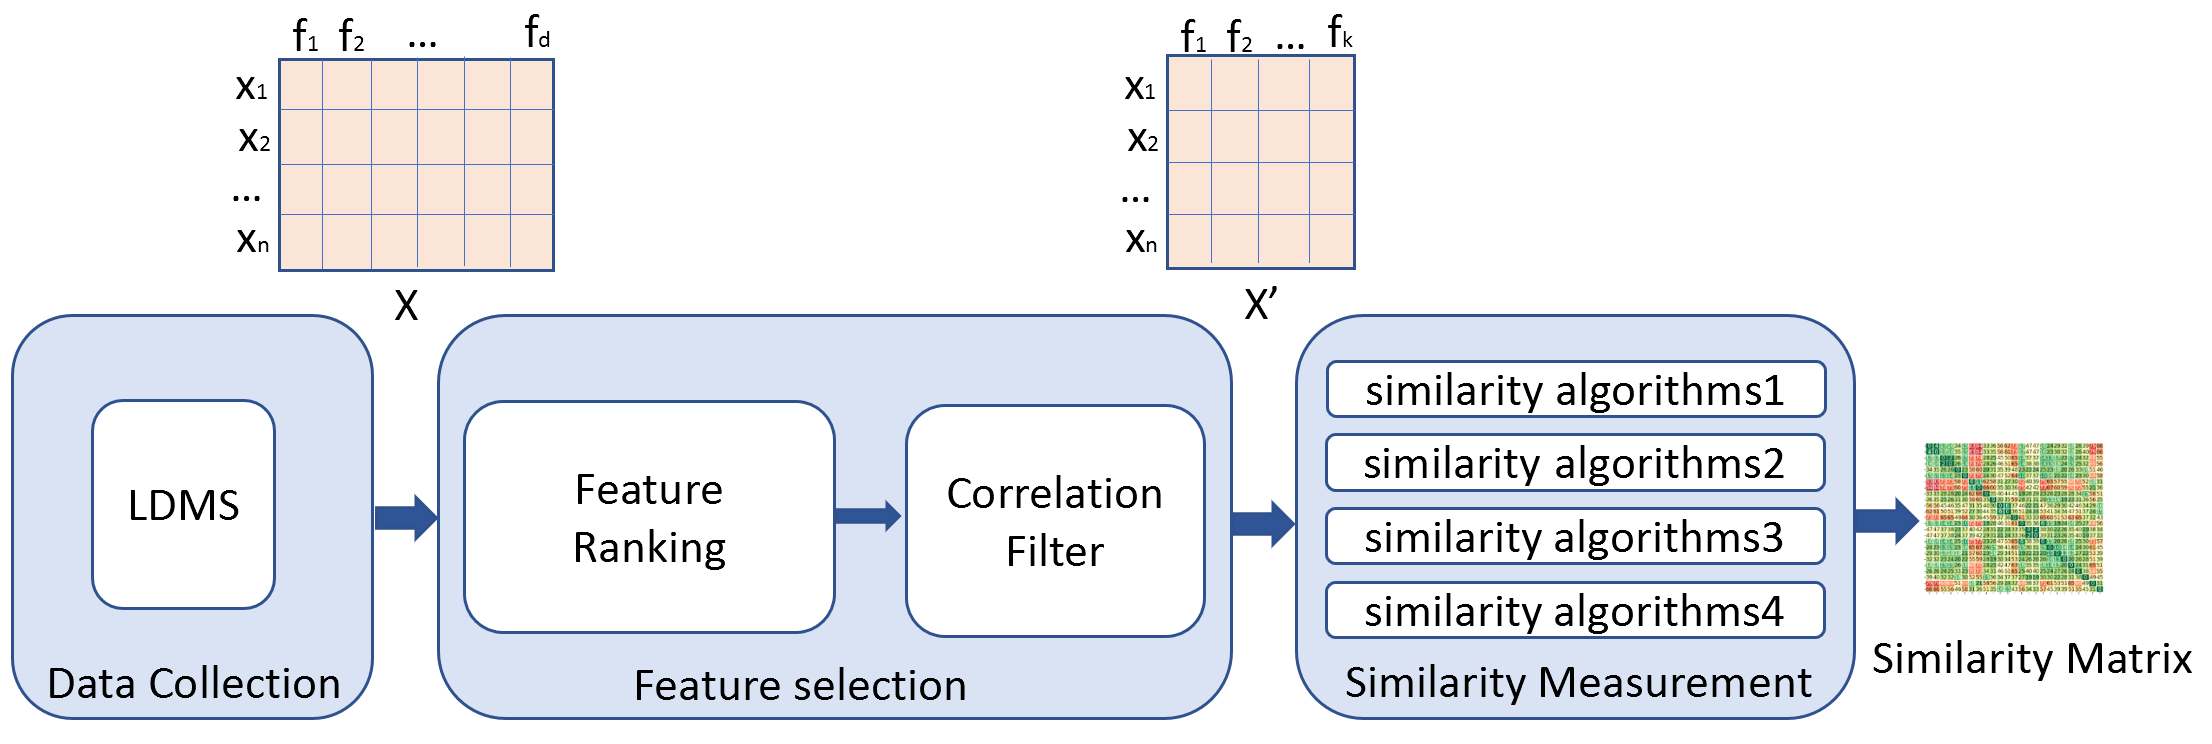
\includegraphics[width=\linewidth]{figs/SimEngine.png}
\caption{\us Architecture }
\label{figs:us}
\end{figure}

\subsection{Similarity and Distance}
\label{sec:Sim}

Evaluating the similarity between proxy and parents is one of the main goals of our work. We define two applications as \emph{similar} if the vectors that represent the applications are a short distance apart, which, in many classification tasks, corresponds to the vectors belonging to the same class. %The similarity is defined using a distance measure. 
After calculating the pairwise distance between each application pair, we get a similarity matrix. % We expect the diagonal of the matrix to be zero distance, as that indicates the distance between the applications and themselves. 
We compare the result of four typical similarity metrics and choose the metric that most accurately correlates known proxy/parent pairs.

\commentout{
\subsubsection{Background}
\todo{this is mostly untested metrics, right?  Why is it here?}
We define two vectors as \emph{similar} if they are a short distance apart, which, in many classification tasks, corresponds to the vectors belonging to the same class.
%of two vectors in space is called similarity. If two vectors are similar, their distance is short, and vice versa.
%In many classification tasks, the samples with short distances are intuitively similar to each other and more likely belong to the same class.
%
%
The most familiar distance metrics are Minkowski distances, where the distance $D$ between two vectors $X$ and $Y$ is defined as $(\sum_{i=1}^n|x_i-y_i|^p)^{1/p}$, which reduces to Manhattan distance at $p=1$ and Euclidean distance at $p=2$~\cite{9distance}. 
%In some scenarios, normalization is needed to overcome the magnitude variant on each feature. 
In high dimensional space, Minkowski distances for small $p$ become less useful because of the curse of dimensionality -- all of the points are about the same distance. Cosine similarity (\S\ref{sec:cos_sim}) has often been used as a way to counteract these drawbacks since the magnitude of vectors is not taken into account. After Z-score standardization, we could consider Pearson correlation, Cosine similarity, and Euclidean distance as equivalent.\avani{previous is unclear} %Minkowski distance is a group of distance metrics, which with some parameters it turns into Manhattan distance, Euclidean distance, and Chebyshev distance. %Undoubtedly, choosing the best parameter is not trivial and depends on use cases. 
The Jaccard Index calculates the similarity and diversity of two sample sets, which are heavily impacted by the size of data. Hamming distance is typically used to compare two binary strings.\avani{why are you telling me about Hamming distance?}

\avani{cut text below for space (see comments in tex)}
%Another big category of distance is statistical distance~\cite{statdis}. Mahalanobis distance~\cite{Mah} is an effective multivariate distance metric that measures the distance between a point (vector) and a distribution or two points from the same distribution. 
%
%It could eliminate the correlation between features. Kullack-leibler divergence~\cite{kullback1951information}, Jensen-Shannon divergence~\cite{endres2003new}, and Wasserstein distance\cite{rubner2000earth} are widely used to minimize the loss function when updating Machine Learning models. 
%
%Obviously, if we use different distance measurements, we would get different distances. Depending on the way we represent the objects of a clustering, we need to find the most appropriate distance metric to achieve the best result for our specific task.
}%------end comment out-------

\subsubsection{Cosine Similarity}
\label{sec:cos_sim}
Cosine similarity compares the angle between the vectors with the vector inner product in vector spaces of multiple dimensions. The inner product can be conceptualized
as the projection of one vector $x_{i}$ in the direction of the other vector $x_{j}$. The calculation relies on the two complementary definitions (algebraic and geometric) for computing the inner product:
\begin{itemize}
\item 
Algebraic Inner Product:
$x_{i}\cdot x_{j}=\sum_{k=1}^{d} x_{ik} x_{jk}$
\item
Geometric Inner Product:
$x_{i}\cdot x_{j}=\|x_{i}\|\|y_{i}\|\cos\theta$
\item
Cosine Similarity:
\begin{equation}
\cos(\theta)=\frac{\sum_{k=1}^{d} x_{ik} x_{jk}}{\|x_{i}\|\|x_{j}\|}
\end{equation}
\end{itemize} 
%Cosine similarity compares the angle between two vectors $x_{i}$ and $x_{j}$ using vector inner product. 
The cosine varies from 1.0 (identical vector direction) to 0.0 (orthogonal vectors), and the degree $\theta$ varies from 0 (similar) to 90 (dissimilar).% indicate similar (the same) and dissimilar respectively. 

\subsubsection{Jensen-Shannon (JS) Divergence}
\label{sec:JS}
Instead of comparing two vectors, we can normalize each vector and think of it as a probability distribution (each event turns into a probability), and then compare the two distributions.
JS divergence~\cite{endres2003new} measures the distance between two probability distributions $P$ and $Q$. JS is a generalization of  Kullback–Leibler (KL) divergence~\cite{kullback1951information}, the relative entropy from distributions $Q$ to $P$, \ie the expectation of the logarithmic difference between the probability distributions $Q$ and $P$. 
\begin{align*}
KL(P|Q)&=\sum_{x} P(x) \log \frac{P(x)}{Q(x)} \\ 
&=-\sum_{x} P(x) \log {Q(x)}+\sum_{x} P(x) \log {P(x)} \\ 
& =\textrm{cross entropy – entropy}
\end{align*}
KL divergence is asymmetric and has no upper bound. Unlike KL divergence, JS divergence is symmetric and returns a value between 0 and 1. %both of which are valuable properties for application comparison. 
JS divergence is defined as 
\begin{equation}
\operatorname{JS}(P \| Q)=\frac{1}{2} KL(P \| M)+\frac{1}{2} KL(Q \| M)
\end{equation}
where $M=\frac{1}{2}(P+Q)$.% JS divergence calculates total KL divergences in two directions to the average.  

\subsubsection{Wasserstein Distance}
\label{sec:wass}
Wasserstein distance\cite{rubner2000earth} can be interpreted as the minimum ``cost'' of transforming a probability distribution $P$ into distribution $Q$, where ``cost'' is measured as the amount of distribution weight that must be moved, multiplied by the distance it has to be moved. Unlike other statistic distances like JS divergence, Wasserstein distance considers both the probability of and the distance between events, thus the order of the events matters. Since Wasserstein distance does not require both measures to be in the same probability space (\ie, two vectors may have different lengths), it can be used to compare application performances across platforms that support a different number of hardware event counts. The $p^{th}$ Wasserstein distance is defined as 
\begin{equation}
W_{p}(P, Q)=\left(\inf _{J \in \mathcal{J}(P, Q)} \int\|x-y\|^{p} d J(x, y)\right)^{1 / p}
\end{equation},
where $\mathcal{J}(P, Q)$ denotes all joint distributions $J$ for $(X,Y)$ that have marginals $P$ and $Q$. Generally, when $p = 1$ and $d = 1$, we compute the first Wasserstein distance between two 1-dimensional distributions, which is also known as earth mover distance. 

\subsubsection{Mahalanobis Distance}
Mahalanobis distance~\cite{Mah} is an effective multivariate distance metric that measures the distance between a point (vector) and a distribution, or two points from the same distribution. 
The Mahalanobis distance~\cite{Mah} between two vectors $x_i$ and $x_j$ from the same distribution is defined as
\begin{equation}d_{M}(x_i, x_j)=\sqrt{(x_i-x_j)^{T} S^{-1}(x_i-x_j)}
\end{equation}, where $S$ is the covariance matrix of the data set. Geometrically, it transforms the data by whitening and normalizing the covariance and computes the ordinary Euclidean distance for the transformed data. Since the Mahalanobis distance accounts for the variance of each variable and the covariance between variables, it is used in areas such as multivariate anomaly detection and imbalanced classification. Note that the Mahalanobis distance requires more samples than features to calculate the covariance matrix. Thus, we reduce features with principal components analysis (PCA) before applying Mahalanobis distance.

\subsection{Feature Selection}
By Occam’s Razor, the simplest model that explains a situation is the correct approach. 
Irrelevant features may increase noise and reduce the accuracy of a model, while adding to latency, storage overhead, and the amount of data processing. There are two classes of algorithms to reduce a feature space: feature extraction and feature selection. 
Feature extraction, which recombines original features into a denser set, retains the overhead of data collection and sacrifices interpretability, so we focus on feature selection.

%Feature extraction is to find a smaller set of new variables, each being a combination of the original features. Because feature extraction still requires collecting all the features and loses interpretability, it is not what we are looking for. 
Feature selection speeds up algorithms, improves accuracy, and enhances comprehensibility~\cite{guyon2003introduction}. 
%\avani{I propose we cut the rest of this paragraph}
%Feature Selection can be categorized into filter methods, wrapper methods, and embedded methods. The filter methods always focus on the intrinsic properties (\eg Variance) of data itself, which are more suitable for unsupervised learning. %Examples of filter methods include Information Gain, Chi-square Test, Fisher’s Score, Correlation Coefficient, Variance Threshold, Mean Absolute Difference, and Dispersion ratio. 
%Wrapper methods evaluate features by applying a selection algorithm and comparing the final value with the target value. They require a greedy search in the feature space. The typical wrapper method is Recursive Feature Elimination\cite{guyon2002gene}. Embedded methods, such as Random Forest\cite{ho1995random}, get the important features while interactively building up the model. Most of the wrapper and embedded feature selection methods are designed for supervised learning. 
To simplify the data collection process and enable cross-platform comparison, we aim to find a concise event subset. \us uses Laplacian score~\cite{he2005laplacian} to rank the important features, combined with the Pearson correlation to remove the correlated features.

\subsubsection{Feature Score}
\label{sec:feature_score}
Consider a data matrix $X$ that has $n$ rows of samples with $d$ dimensions $x_{1},...,x_{n}$. The columns of $X$ are the features $f_{1},...f_{d}$. Our goal is to find the subset of $k$ important features which preserve the similarity structure of the matrix $X$. 

%Since we lack ground truth for the class label for each application, the filter method of feature selection is more suitable.
Since we are only interested in keeping the similarity relationship between the proxy/parent application pair points, but not concerned about the dissimilarity of non-proxy/parent application pair points, neighbor embedding is the perfect unsupervised method for this task. We choose a graph-based feature ranking technology called Laplacian score~\cite{he2005laplacian} to compute the importance of features.  Laplacian score builds a nearest neighbor graph for application points and seeks those features that respect local graph structure. In our case, these features help preserve the neighbor similarity between proxy and parent applications.  

The Laplacian score of the $r^\textrm{th}$ feature can be expressed as:
\begin{equation}L_{r}=\frac{\widetilde{\mathbf{f}}_{r}^{T} L \widetilde{\mathbf{f}}_{r}}{\widetilde{\mathbf{f}}_{r}^{T} \widetilde{\mathbf{f}_{r}}}
\end{equation}
, or in a more understandable way:
\begin{equation}
L_{r}=\frac{\Sigma_{i j}\left(f_{r i}-f_{r j}\right)^{2} S_{i j}}{\operatorname{Var}\left(\mathbf{f}_{r}\right)}
\end{equation} , where $f_r$ is the $r^\textrm{th}$ feature, and $S_{i j}$ is the weight matrix. An element $S_{i j}$ will only have a nonzero value $S_{i j}=e^{-\frac{\left\|\mathrm{x}_{i}-\mathrm{x}_{j}\right\|^{2}}{2t^{2}}}$ when $i$ and $j$ are neighbors, otherwise the value of that entry is zero. $t$ is a user-defined bandwidth, with $1$ as a default value. The denominator indicates the variance of the $r^\textrm{th}$ feature; larger values correlate to more information represented. The numerator indicates the sum of feature value differences within the points' neighbors; here, the smaller the Laplacian score is, the more important the feature is. Finally, we get the ranked features sorted by Laplacian score.

Since features are evaluated separately in the Laplacian score, if we select features with the smallest Laplacian score, some redundant features may be included. To select an informative set of important features in order to optimize combination performance, we introduce the correlation filter.

\subsubsection{Correlation Filter}
When a group of features are highly correlated, we only need to include one in our selection. A broadly used correlation measure is the Pearson correlation coefficient (PCC). PCC measures the linear correlation between two variables $f_{i}, f_{j}$. 
\begin{equation}
\rho_{f_{i}, f_{j}}=\frac{\operatorname{cov}(f_{i}, f_{j})}{\sigma_{f_{i}} \sigma_{f_{j}}}
\end{equation}
where $\operatorname{cov}$ is the covariance and $\sigma_{f_{i}}$is the standard deviation of $f_{i}$.
PCC has a value between +1 and -1, where +1 is a total positive linear correlation, 0 is no linear correlation, and -1 is a total negative linear correlation. We choose a PCC threshold of 0.9 because we want to keep reasonable number of important features while removing strongly correlated ones.  

We calculate the pairwise PCC for all ranked features and fetch features one by one from the ranked feature to our important feature subset. Each time we select one feature, we remove the redundant features with PCC $> 0.9$ or $< -0.9$ from the remaining features. We stop collecting features when there are no more features in the feature pool. %we obtain a pre-selected number, or when there are no more features in the feature pool.

Note that the PCC can evaluate only a linear relationship between two continuous variables; we will investigate more correlation methods in future work.